\documentclass{article} % say

\usepackage{tikz}
\usetikzlibrary{
	arrows,
	decorations.pathmorphing,
	backgrounds,
	positioning,fit,
	petri
}

\begin{document}

Styles, labeled circles in a row.

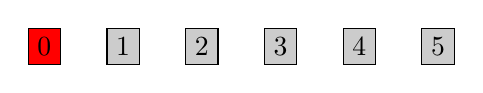
\begin{tikzpicture}
[place/.style={circle,draw=blue!50,fill=blue!20,thick},
transition/.style={rectangle,draw=black!50,fill=black!20,thick},
bit/.style={rectangle,draw=black,fill=black!20,thin}]
\node at ( 0,0) [bit,fill=red] {$0$};
\node at ( 1,0) [bit] {$1$};
\node at ( 2,0) [bit] {$2$};
\node at ( 3,0) [bit] {$3$};
\node at ( 4,0) [bit] {$4$};
\node at ( 5,0) [bit] {$5$};
\end{tikzpicture}

Looped series of bit boxes.

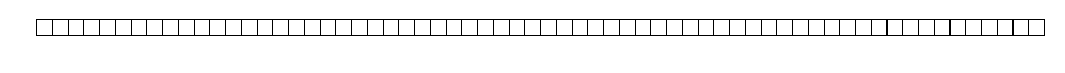
\begin{tikzpicture}
\tikz \foreach \x in {63,62,...,0}
	\draw (0.2*\x,0) +(-.1,-.1) rectangle ++(.1,.1);


\end{tikzpicture}

\end{document}

